\chapter{Problem 3 --- Surat dari Tetangga (Orang 1: kriteria 1--5; Orang 2: kriteria 6)}

> Draf bagian laporan M2. Bukti: \texttt{make demo-\allowbreak{}m2-\allowbreak{}p3} (\texttt{docs/\allowbreak{}evidence/\allowbreak{}m2/\allowbreak{}p3-\allowbreak{}latest.\allowbreak{}log}), \texttt{make demo-\allowbreak{}p1} (M1, kini > memakai dead-letter store), test \texttt{services/\allowbreak{}aggregator/\allowbreak{}internal/\allowbreak{}\{sources,\allowbreak{}dlq,\allowbreak{}poller,\allowbreak{}mapping,\allowbreak{}api\}}, > \texttt{internal/\allowbreak{}ports/\allowbreak{}repotest} (\texttt{runUnprocessed}), dan \texttt{services/\allowbreak{}pvmbg-\allowbreak{}mock/\allowbreak{}internal/\allowbreak{}pvmbg/\allowbreak{}m2\_\allowbreak{}test.\allowbreak{}go}. > Bagian kriteria 6 (\texttt{POST /\allowbreak{}field-\allowbreak{}reports}) ditulis Orang 2.


\section{Identifikasi masalah}

{\small
\begin{longtable}{@{}>{\raggedright\arraybackslash}p{0.112\linewidth}>{\raggedright\arraybackslash}p{0.411\linewidth}>{\raggedright\arraybackslash}p{0.411\linewidth}@{}}
\toprule
\textbf{Kriteria} & \textbf{Persoalan} & \textbf{Nama dalam literatur} \\
\midrule
\endhead
2 & Pesan yang gagal diproses harus disimpan, bukan dibuang atau dicoba terus-menerus; kegagalan sementara harus dibedakan dari kegagalan permanen & \emph{Dead letter queue / dead letter channel} (Hohpe \& Woolf, \emph{Enterprise Integration Patterns}); \emph{transient vs permanent fault}, \emph{retry with exponential backoff} \\
3 & Satu pesan rusak (terpotong, bersarang sangat dalam, UTF-8 rusak, sangat besar) membuat parser gagal atau proses kehabisan memori, lalu restart berulang dan memblokir pesan lain & \emph{Poison message / poison pill}; \emph{head-of-line blocking}; \emph{crash loop} \\
4 & Setelah sistem disesuaikan, pesan lama diproses ulang: tidak boleh ganda dan tidak boleh menimpa data yang lebih baru & \emph{Replay / reprocessing} dengan \emph{idempotent consumer}; \emph{per-key ordering} (\emph{ordered delivery per entity}) \\
1 & Skema mitra berubah tanpa koordinasi; sistem harus tahu mana yang boleh diterima & \emph{Schema evolution}, \emph{tolerant reader} (Fowler), kompatibilitas \emph{backward/forward} \\
6 & Laporan Tim Lapangan harus diterima walau pemrosesan hilir lambat atau mati, tidak boleh hilang setelah dijawab 202 walau penerimanya mati, dan tidak boleh diproses dua kali walau klien mengulang & \emph{Asynchronous request--reply} / \emph{request acknowledgement} (202 Accepted), \emph{durable message queue} (\emph{store-and-forward}), \emph{at-least-once delivery} + \emph{idempotent receiver} (Hohpe \& Woolf) = \emph{effectively-once}; \emph{exactly-once processing} dengan \emph{transactional consume--transform--produce} (Kafka KIP-98/KIP-447); \emph{zombie fencing} \\
\bottomrule
\end{longtable}
}

\section{Kebijakan perubahan skema (kriteria 1)}

Kebijakan M1 dipertahankan dan dinyatakan di komentar paket \texttt{services/\allowbreak{}aggregator/\allowbreak{}internal/\allowbreak{}mapping/\allowbreak{}raw.\allowbreak{}go}:


{\small
\begin{longtable}{@{}>{\raggedright\arraybackslash}p{0.307\linewidth}>{\raggedright\arraybackslash}p{0.296\linewidth}>{\raggedright\arraybackslash}p{0.331\linewidth}@{}}
\toprule
\textbf{Perubahan} & \textbf{Sikap} & \textbf{Alasan} \\
\midrule
\endhead
Field baru (tipe apa pun) & \textbf{diterima otomatis} $\rightarrow$ \texttt{attributes} & Tidak mengubah arti field kanonik; tidak ada data yang dibuang \\
Field non-kanonik hilang atau berganti tipe & \textbf{diterima otomatis} & Disimpan apa adanya di \texttt{attributes}; tidak ada aturan pemetaan yang bergantung padanya \\
Urutan / format field & \textbf{diterima otomatis} & Record dibaca sebagai peta, bukan posisi \\
Field kanonik di-\emph{rename}, dihapus, dipindah, atau berganti tipe; nilai enum baru & \textbf{tidak diterima} $\rightarrow$ \emph{parked} \texttt{schema\_\allowbreak{}incompatible} & Menebak arti sama dengan risiko severity atau lokasi yang salah pada peringatan bencana \\
Byte yang tidak bisa dibaca & \textbf{tidak diterima} $\rightarrow$ \emph{parked} \texttt{malformed} (\emph{retrying} bila terpotong di jalan) & Tidak ada isi yang bisa dipetakan \\
\bottomrule
\end{longtable}
}

Mock PVMBG mendapat mode baru di \texttt{POST /\allowbreak{}admin/\allowbreak{}schema-\allowbreak{}version} (\texttt{\{"mode":"incompatible"\}} / \texttt{\{"version":3\}} / pilihan \texttt{\{"incompatible":["rename",\allowbreak{}"type\_\allowbreak{}change",\allowbreak{}"drop\_\allowbreak{}required"]\}}): \texttt{alert\_\allowbreak{}level} $\rightarrow$ \texttt{level}, \texttt{reported\_\allowbreak{}at} ISO $\rightarrow$ angka Unix, \texttt{volcano\_\allowbreak{}id} hilang (kodenya pindah ke \texttt{location.\allowbreak{}volcano\_\allowbreak{}code}). Laporan lama tetap berbentuk lama, seperti versi API baru di dunia nyata. \texttt{POST /\allowbreak{}admin/\allowbreak{}malformed} membuat pesan rusak.


\section{Mekanisme}

\begin{figure}[H]\centering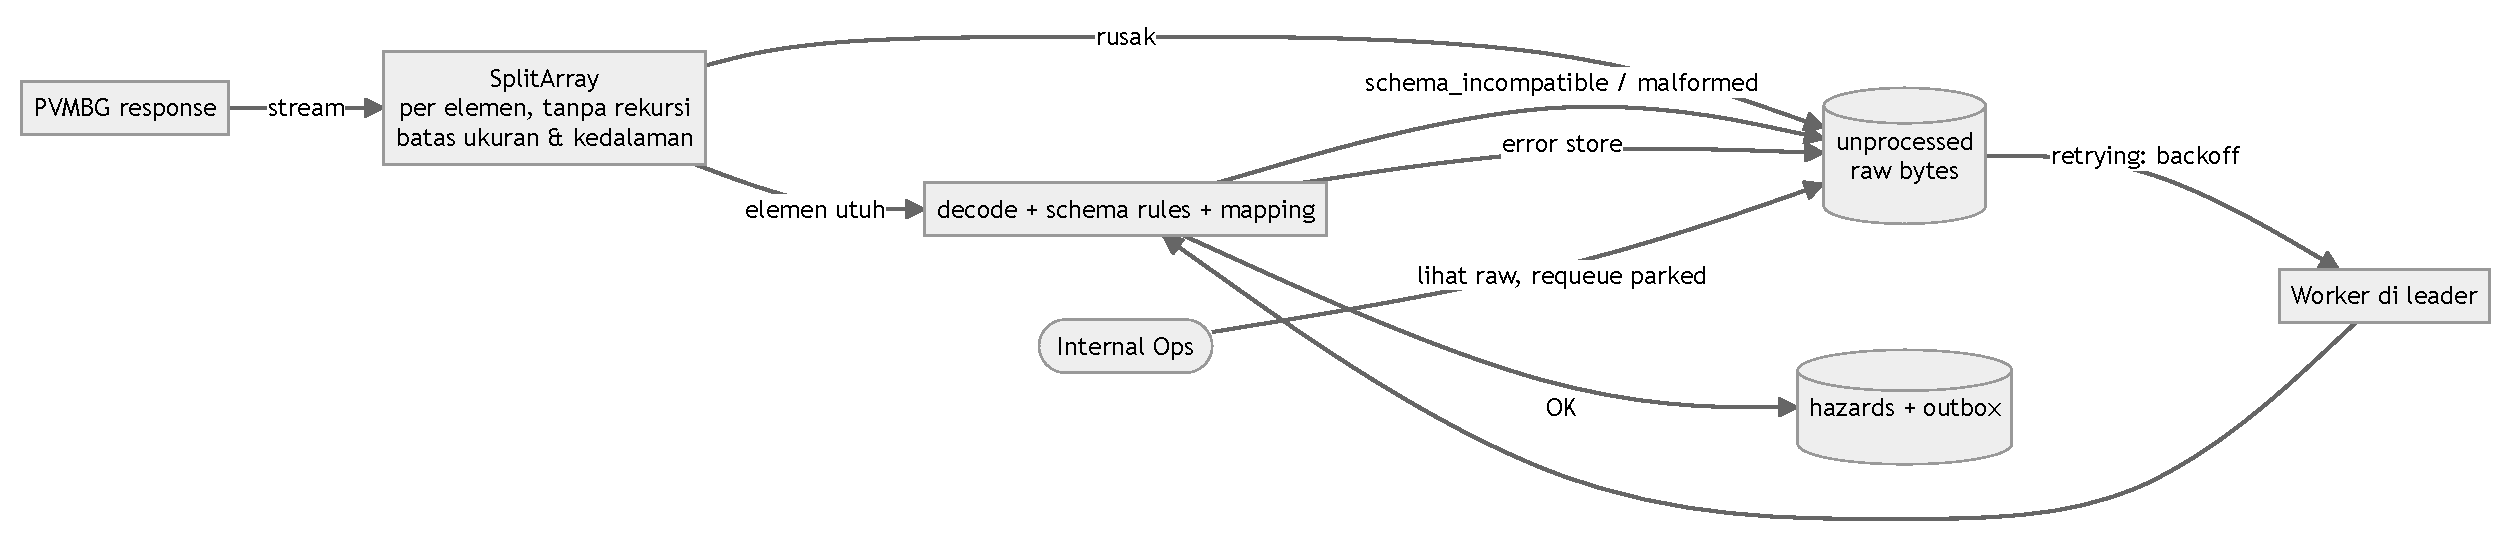
\includegraphics[width=\linewidth,height=0.82\textheight,keepaspectratio]{fig/m5.pdf}\end{figure}

\begin{enumerate}
\item \textbf{Membaca tanpa bisa dijatuhkan} (\texttt{sources/\allowbreak{}split.\allowbreak{}go}). Respons dibaca sebagai \emph{stream} dan dipecah per elemen array tanpa di-\emph{decode}: kedalaman dihitung dengan penghitung (tanpa rekursi), satu elemen paling banyak \texttt{MESSAGE\_\allowbreak{}MAX\_\allowbreak{}BYTES} (1 MiB) ditahan di memori, UTF-8 diperiksa eksplisit (\texttt{encoding/\allowbreak{}json} diam-diam mengganti byte rusak dengan U+FFFD). Elemen rusak dikembalikan bersama masalahnya; elemen di sekitarnya tetap diproses. Tidak ada \texttt{panic} yang mungkin dari input.
\item \textbf{Dead-letter store} (\texttt{internal/\allowbreak{}dlq}, tabel \texttt{unprocessed} di Canonical Store). Setiap pesan gagal disimpan dengan \textbf{byte persis} yang diterima, \texttt{reason}, \texttt{source}, \texttt{received\_\allowbreak{}at}, \texttt{kind}, \texttt{record\_\allowbreak{}key}, \texttt{attempts}, \texttt{status}. \texttt{message\_\allowbreak{}id} = sha256(source, kind, bytes), jadi pesan yang diambil ulang oleh jendela overlap polling tidak tersimpan dua kali.
\item \textbf{Dua perlakuan berbeda} (kriteria 2):
\begin{itemize}
\item \emph{retrying} (\texttt{retryable: true}): kegagalan yang bisa hilang sendiri --- tulis ke store gagal, peringatan tsunami yang event-nya belum datang (\texttt{dependency\_\allowbreak{}missing}), elemen terpotong di jalan (sumber dipoll ulang dari watermark yang sama). Worker di leader mencoba ulang dengan \emph{exponential backoff} 2 s \ldots{} 120 s, maksimum 8 kali, lalu \emph{parked} \texttt{retry\_\allowbreak{}exhausted}. Elemen terpotong selesai sendiri begitu record utuhnya tersimpan.
\item \emph{parked} (\texttt{retryable: false}): \texttt{schema\_\allowbreak{}incompatible} dan \texttt{malformed}. \textbf{Tidak pernah dicoba otomatis} (mencoba lagi byte yang sama dengan kode yang sama pasti gagal). Menunggu perubahan sistem lalu \emph{requeue} oleh Internal Ops.
\end{itemize}
\item \textbf{Watermark tidak tertahan pesan buruk}: kursor polling maju melewati pesan yang sudah aman di dead-letter store, sehingga satu pesan rusak tidak membuat sumber diambil ulang terus (head-of-line blocking).
\item \textbf{Penyesuaian sistem tanpa kode baru} (\texttt{mapping/\allowbreak{}rules.\allowbreak{}go}): aturan deklaratif per sumber --- \texttt{rename} (termasuk path bersarang) dan \texttt{coerce} (\texttt{unix\_\allowbreak{}seconds\_\allowbreak{}to\_\allowbreak{}rfc3339}, \texttt{number\_\allowbreak{}to\_\allowbreak{}string}, \ldots{}) --- dimuat dari ConfigMap \texttt{aggregator-\allowbreak{}schema-\allowbreak{}rules}. Aturan hanya \textbf{mengisi field kanonik yang kosong}, jadi record skema lama tidak berubah. Aturan tidak valid menghentikan start-up (pod tidak Ready, rollout berhenti), bukan diabaikan diam-diam. Contoh penyesuaian PVMBG v3: \texttt{deploy/\allowbreak{}schema-\allowbreak{}rules/\allowbreak{}pvmbg-\allowbreak{}v3.\allowbreak{}json}.
\item \textbf{Pemrosesan ulang} (kriteria 4): \texttt{POST /\allowbreak{}internal/\allowbreak{}ops/\allowbreak{}unprocessed/\allowbreak{}reprocess} memindahkan pesan \emph{parked} ke \emph{retrying}. Worker memprosesnya dengan \textbf{kode yang sama} dengan jalur normal (\texttt{PVMBGSource.\allowbreak{}process}), urut kedatangan (\texttt{seq}).
\begin{itemize}
\item \emph{Tanpa duplikat}: \texttt{hazard\_\allowbreak{}id} deterministik dan \texttt{Upsert} idempoten; pesan yang ternyata sudah tersimpan menghasilkan \texttt{unchanged}.
\item *Urutan per \texttt{source\_\allowbreak{}ref\_\allowbreak{}id}*: selama ada pesan terbuka untuk record yang sama (sumber + kind + \texttt{record\_\allowbreak{}key}), pesan baru record itu ikut masuk antrean dengan alasan \texttt{ordered\_\allowbreak{}after: <id>} dan worker hanya memproses pesan terdepan per record. Pesan lama yang pulih tidak bisa menimpa data yang lebih baru (\texttt{TestIncompatibleChangeRecoversAfterAdjustmentInOrderWithoutDuplicates}: VR-1 v1 diproses sebelum v2, hasil akhir AWAS v2).
\end{itemize}
\item \textbf{Hanya Internal Ops} (kriteria 5): \texttt{/\allowbreak{}internal/\allowbreak{}ops/\allowbreak{}*} hanya menerima \texttt{Authorization: Bearer <AGGREGATOR\_\allowbreak{}OPS\_\allowbreak{}TOKEN>}. Kredensial Client-Facing API (\texttt{X-\allowbreak{}Service-\allowbreak{}Key}) dan token auditor ditolak (401/403). Auditor mendapat \texttt{/\allowbreak{}internal/\allowbreak{}audit/\allowbreak{}unprocessed} (Lampiran A) yang hanya memuat metadata, tanpa isi pesan. \texttt{GET /\allowbreak{}internal/\allowbreak{}quarantine} M1, yang terbuka untuk service key, dihapus.
\end{enumerate}

\section{Alternatif yang dipertimbangkan}

{\small
\begin{longtable}{@{}>{\raggedright\arraybackslash}p{0.297\linewidth}>{\raggedright\arraybackslash}p{0.649\linewidth}@{}}
\toprule
\textbf{Alternatif} & \textbf{Konsekuensi} \\
\midrule
\endhead
Buang pesan buruk dan catat di log & Melanggar kriteria 2; isi tidak bisa diproses ulang \\
DLQ sebagai topic Kafka & Wajar untuk alur push, tetapi butuh konsumen DLQ, penyimpanan status, dan akses terkontrol tambahan; tabel di store yang sudah dimiliki Aggregator memberi query, status, dan transaksi dengan fencing tanpa komponen baru \\
Retry semua kegagalan dengan backoff & Pesan rusak permanen mengisi antrean retry selamanya dan menyamarkan masalah nyata \\
Coba tebak (\texttt{level} mungkin \texttt{alert\_\allowbreak{}level}) & Cepat, tetapi tebakan salah pada peringatan bencana lebih berbahaya daripada keterlambatan; penyesuaian tetap butuh keputusan manusia \\
Parser JSON standar untuk seluruh respons & Satu elemen buruk menggagalkan seluruh batch; kedalaman ekstrem dan ukuran besar memakan memori \\
\bottomrule
\end{longtable}
}

\section{Batasan yang disadari}

\begin{itemize}
\item Pesan melebihi \texttt{MESSAGE\_\allowbreak{}MAX\_\allowbreak{}BYTES} disimpan \textbf{1 MiB pertama} + ukuran aslinya (bukan ``utuh''), agar satu pesan tidak bisa menghabiskan memori atau tabel. Pesan seperti itu tidak bisa dipulihkan dengan aturan skema; perlu perubahan batas.
\item Watermark hanya maju oleh record yang waktunya bisa dibaca. Bila sumber mengubah tipe \texttt{reported\_\allowbreak{}at}, record baru diambil ulang tiap siklus sampai aturan dipasang (tidak ganda karena \texttt{message\_\allowbreak{}id}), dengan biaya bandwidth.
\item Elemen terpotong tanpa \texttt{report\_\allowbreak{}id} yang terbaca tidak bisa dikaitkan dengan record utuhnya; ia di-\emph{parked} \texttt{retry\_\allowbreak{}exhausted} setelah 8 percobaan (datanya sendiri tetap masuk dari respons berikutnya).
\item Aturan skema hanya \texttt{rename} dan \texttt{coerce}. Perubahan makna atau satuan butuh kode baru (versi Aggregator baru, rolling update tanpa downtime, lalu requeue --- jalurnya sama).
\end{itemize}

\section{Bukti per kriteria}

{\small
\begin{longtable}{@{}>{\raggedright\arraybackslash}p{0.161\linewidth}>{\raggedright\arraybackslash}p{0.785\linewidth}@{}}
\toprule
\textbf{Kriteria} & \textbf{Bukti} \\
\midrule
\endhead
1 & \texttt{make demo-\allowbreak{}m2-\allowbreak{}p3} langkah 1 (field baru diterima otomatis ke \texttt{attributes}) dan 4 (3 laporan tidak kompatibel di-\emph{parked} dengan byte persis, tidak ditebak). Diulang 22 Nov di storage sharded: \texttt{p3-\allowbreak{}sharded-\allowbreak{}20261122.\allowbreak{}log}. lulus \\
2 & langkah 2: \texttt{too\_\allowbreak{}deep}, \texttt{invalid\_\allowbreak{}utf8}, \texttt{too\_\allowbreak{}large} \emph{parked} (attempts tidak bertambah), elemen terpotong \emph{retrying} $\rightarrow$ \emph{resolved} sendiri tanpa intervensi (22 Nov, sharded). lulus \\
3 & langkah 2: restart count Aggregator tidak berubah; laporan valid yang dikirim bersama pesan rusak tetap tersimpan (22 Nov, sharded). lulus \\
4 & langkah 5: aturan PVMBG v3 dipasang lewat rolling update, requeue, ketiga laporan tersimpan, \texttt{count(*) -\allowbreak{} count(DISTINCT source\_\allowbreak{}ref\_\allowbreak{}id) =\allowbreak{} 0}. lulus di k3s pada 14 Nov (\texttt{p3-\allowbreak{}latest.\allowbreak{}log}, store tunggal). Pada ulangan 22 Nov di storage sharded, rolling update untuk memasang aturan tidak selesai: pod Aggregator baru tidak dapat menjangkau Kafka karena NetworkPolicy node-a belum menerima IP pod baru setelah node itu di-reset paksa (lihat §5). Langkah ini tidak bergantung pada jenis storage. \\
5 & langkah 3: \texttt{X-\allowbreak{}Service-\allowbreak{}Key} 401, service key sebagai Bearer 403, token audit 403, token Ops 200 (22 Nov, sharded). lulus \\
6 & \texttt{make demo-\allowbreak{}m2-\allowbreak{}field-\allowbreak{}reports} (\texttt{docs/\allowbreak{}evidence/\allowbreak{}m2/\allowbreak{}p3-\allowbreak{}field-\allowbreak{}reports-\allowbreak{}latest.\allowbreak{}log}; run pengembangan: \texttt{p3-\allowbreak{}field-\allowbreak{}reports-\allowbreak{}kind.\allowbreak{}log}): pemroses mati, 20$\times$202 p50 36 ms / p95 298 ms; 5 retry $\rightarrow$ \texttt{report\_\allowbreak{}id} sama; semua pod client-api dibunuh setelah 202; pemroses dibunuh di tengah transaksi; 40 diterima $\rightarrow$ 40 record di \texttt{field-\allowbreak{}reports.\allowbreak{}processed}, 40 berbeda. Test: \texttt{client-\allowbreak{}api/\allowbreak{}internal/\allowbreak{}api/\allowbreak{}fieldreports\_\allowbreak{}test.\allowbreak{}go}, \texttt{field-\allowbreak{}reports/\allowbreak{}internal/\allowbreak{}processor/\allowbreak{}processor\_\allowbreak{}test.\allowbreak{}go} (duplikat, restart, zombie) \\
\bottomrule
\end{longtable}
}

\section{Kriteria 6 --- \texttt{POST /\allowbreak{}field-\allowbreak{}reports} (Orang 2)}

\subsection{Persoalan}

Tim Lapangan mengirim laporan dari lokasi dengan sinyal yang mungkin hanya cukup untuk satu kali kirim. Ada tiga hal yang dapat merusaknya:


\begin{enumerate}
\item \textbf{Hilir lambat atau mati.} Bila 202 menunggu pemrosesan, satu pemroses yang lambat membuat semua pengirim menunggu sampai timeout dan mengulang. Inilah alasan pola \emph{asynchronous request--reply}: terima dulu, proses kemudian.
\item \textbf{Penerima mati setelah 202.} Laporan yang hanya ada di memori proses penerima ikut hilang. Masalah ini disebut \emph{durability before acknowledgement}: yang boleh dijawab ``diterima'' hanyalah yang sudah tersimpan tahan lama.
\item \textbf{Pengiriman ulang.} Jaringan dapat menelan balasan 202. Klien yang benar akan mengirim ulang, dan sistem melihat laporan yang sama dua kali. Jaminan \emph{at-least-once} hanya aman bila penerimanya \emph{idempotent receiver}. Sebaliknya, pemroses yang mati di tengah pekerjaan akan mengulang input yang sudah setengah diproses, dan ini juga memerlukan \emph{exactly-once processing}.
\end{enumerate}

\subsection{Mekanisme}

\begin{lstlisting}
Tim Lapangan --POST + Idempotency-Key--> client-api --produce acks=all--> [field-reports] --202-->
                                                         (idempoten)          |
                       services/field-reports: consume --(transaksi Kafka)--> [field-reports.processed] + commit offset
\end{lstlisting}

\begin{itemize}
\item \textbf{Kunci idempotensi dan identitas laporan.} Klien mengirim \texttt{Idempotency-\allowbreak{}Key}, lalu \texttt{report\_\allowbreak{}id =\allowbreak{} sha256(client\_\allowbreak{}id,\allowbreak{} key)}. Pengulangan dengan kunci yang sama menghasilkan \texttt{report\_\allowbreak{}id} dan key Kafka yang sama, sehingga masuk ke partisi yang sama dengan urutan yang terjaga.
\item \textbf{Tahan lama sebelum 202.} client-api memanggil \texttt{ProduceSync} dengan \texttt{acks=\allowbreak{}all} dan producer idempoten. Producer idempoten mencegah satu produce yang diulang oleh library tertulis dua kali di partisi. 202 baru dikirim setelah broker mengonfirmasi. client-api tidak menyimpan apa pun sesudahnya, jadi pod-nya boleh mati kapan saja. Bila broker tidak menjawab dalam 5 s, klien mendapat 503 dan mengulang dengan kunci yang sama. Pemroses hilir tidak ada di jalur ini: 202 tetap cepat walau pemroses mati (demo langkah 1: p95 0,30 s dengan pemroses 0 replika).
\item \textbf{Pemrosesan exactly-once.} \texttt{services/\allowbreak{}field-\allowbreak{}reports} memakai \texttt{kgo.\allowbreak{}GroupTransactSession}. Dalam \textbf{satu transaksi}, pemroses menulis record hasil ke \texttt{field-\allowbreak{}reports.\allowbreak{}processed} dan meng-commit offset input. Akibatnya:
\begin{itemize}
\item bila pemroses mati sebelum commit, transaksi di-abort, keluaran tidak terlihat oleh pembaca \texttt{read\_\allowbreak{}committed}, dan input dibaca ulang;
\item bila mati sesudah commit, tidak ada yang perlu diulang.
\end{itemize}
\item \textbf{Dedup lintas pengulangan klien.} Laporan yang sama yang dikirim dua kali adalah dua record input. Pemroses menyimpan set \texttt{report\_\allowbreak{}id} yang sudah diproses dan melewati yang kedua. Set ini dibangun ulang saat start dari topic \emph{compacted} \texttt{field-\allowbreak{}reports.\allowbreak{}processed} (read\_committed, sampai \emph{last stable offset}), sebelum bergabung ke group. Karena itu pemroses tidak membutuhkan database sendiri.
\item \textbf{Zombie.} Instance lama yang masih hidup (beku, terpartisi) di-fence dua kali:
\begin{itemize}
\item oleh \texttt{transactional.\allowbreak{}id} yang sama, karena instance baru menaikkan epoch sehingga commit instance lama ditolak \texttt{PRODUCER\_\allowbreak{}FENCED};
\item oleh generasi consumer group, karena commit offset instance lama ditolak setelah rebalance.

Setiap batch yang gagal mengakhiri sesi; sesi baru (epoch baru) dibuat setelah set dedup dibangun ulang. Test
\texttt{TestZombieIsFencedAndNothingIsProcessedTwice} membuktikannya.
\end{itemize}
\end{itemize}

\subsection{Jaminan pengiriman (butir ``Di laporan'' 4)}

\emph{*At-least-once dari klien ke broker, exactly-once dari broker ke hasil olahan, jadi *effectively exactly-once} per \texttt{report\_\allowbreak{}id}.** Rinciannya:


\begin{itemize}
\item Laporan yang mendapat 202 sudah ada di log Kafka yang tahan lama, sehingga \textbf{tidak hilang} walau client-api atau pemroses mati.
\item Laporan yang tidak mendapat 202 menjadi tanggung jawab klien: ia mengulang dengan kunci yang sama.
\item Setiap \texttt{report\_\allowbreak{}id} muncul \textbf{tepat sekali} di \texttt{field-\allowbreak{}reports.\allowbreak{}processed} (read\_committed).
\end{itemize}

Bukti (\texttt{make demo-\allowbreak{}m2-\allowbreak{}field-\allowbreak{}reports}):


\begin{enumerate}
\item Pemroses di-\emph{scale} ke 0; 20 laporan semuanya 202 (p95 0,30 s).
\item Lima laporan dikirim ulang dengan kunci sama; \texttt{report\_\allowbreak{}id} tetap sama.
\item Semua pod client-api dibunuh (\texttt{-\allowbreak{}-\allowbreak{}grace-\allowbreak{}period=\allowbreak{}0 -\allowbreak{}-\allowbreak{}force}) tepat setelah 20 laporan berikutnya mendapat 202.
\item Pemroses dihidupkan dengan jeda 300 ms per laporan, lalu dibunuh di tengah transaksi.
\item Topic hasil berisi **40 record untuk 40 \texttt{report\_\allowbreak{}id} berbeda**, sama dengan jumlah \texttt{report\_\allowbreak{}id} yang mendapat 202. Log memperlihatkan \texttt{dedup\_\allowbreak{}set\_\allowbreak{}rebuilt} dan \texttt{field\_\allowbreak{}report\_\allowbreak{}duplicate\_\allowbreak{}skipped} untuk retry.
\end{enumerate}

\subsection{Alternatif}

{\small
\begin{longtable}{@{}>{\raggedright\arraybackslash}p{0.321\linewidth}>{\raggedright\arraybackslash}p{0.625\linewidth}@{}}
\toprule
\textbf{Alternatif} & \textbf{Konsekuensi} \\
\midrule
\endhead
Proses sinkron lalu jawab 200 & 202 tidak lagi cepat ketika hilir lambat atau mati; klien timeout dan mengulang sehingga beban berlipat. Ditolak. \\
Antrean di memori client-api (channel) lalu 202 & Laporan hilang bila pod mati setelah 202. Melanggar kriteria. \\
Tulis ke database client-api lalu \emph{outbox} & Benar, tetapi client-api butuh storage sendiri (aturan satu storage satu pemilik, PV, backup), padahal Kafka sudah tahan lama dan sudah dipakai. \\
Consumer at-least-once + dedup di database & Dedup tetap butuh storage, dan ada celah antara ``tulis hasil'' dan ``commit offset''. Transaksi Kafka menutup celah itu tanpa storage tambahan. \\
Dedup di client-api (cek kunci sebelum produce) & client-api stateless dengan banyak replika; dedup di sana butuh state bersama dan tetap racy. Dedup di pemroses (satu writer per partisi) cukup dan sederhana. \\
\bottomrule
\end{longtable}
}

\subsection{Batasan yang disadari}

\begin{itemize}
\item Broker Kafka satu node (\texttt{replication.\allowbreak{}factor=\allowbreak{}1}, keputusan M1). \texttt{acks=\allowbreak{}all} berarti ditulis ke log broker. Bila disk node broker hilang, laporan yang belum diproses ikut hilang. Replikasi broker ($\ge$ 3 broker) adalah perbaikan berikutnya dan di luar kapasitas cluster 2 VM.
\item Set dedup ada di memori pemroses dan dibangun ulang dari topic compacted. Waktu start sebanding dengan jumlah \texttt{report\_\allowbreak{}id} unik (kecil untuk PoC).
\item Kunci yang sama dengan isi berbeda diperlakukan sebagai pengulangan: isi pertama yang menang. Ini tidak dideteksi sebagai konflik.
\item \texttt{GET /\allowbreak{}v1/\allowbreak{}field-\allowbreak{}reports/\allowbreak{}\{id\}} hanya mengenal laporan yang \textbf{sudah diproses}. Laporan yang diterima tetapi belum diproses menghasilkan 404 sampai diproses.
\end{itemize}
